\documentclass[11pt]{book}

% Cover Variables
	\newcommand{\ctitle}{Tittle}
	\newcommand{\cautor}{Autor}
% TOC Variables
	\newcommand{\toctitle}{Table of Content}
	\newcommand{\toccount}{2}
% Chapter Variables
	\newcommand{\chvar}{Chapter -}

\input{\string~/Projects/common/.style.tex}

\input{\string~/Projects/common/.math.tex}

\input{\string~/Projects/common/.header.tex}
	\pagestyle{fancy}
	\fancyhf{}
	\fancyhead[RE, LO]{\textbf{\chaptername\ \thechapter\  --\ \leftmark}}
	\fancyfoot[LE, RO]{\textbf{Page \thepage}}
	\fancyfoot[LO, RE]{\text{\rightmark}}
	
\input{\string~/Projects/common/.toc.tex}

% figure support
\usepackage{import}
\usepackage{xifthen}
\pdfminorversion=7
\usepackage{pdfpages}
\usepackage{transparent}
\newcommand{\incfig}[1]{%
	\def\svgwidth{\columnwidth}
	\import{./figures/}{#1.pdf_tex}
}

\pdfsuppresswarningpagegroup=1

\begin{document}
	% Spacing 
	\input{\string~/Projects/common/.begin.tex}

	\section{TD Math - Intégrales Doubles}

	\subsection{Exercise 56}

	On note $\ds{T}$ le domaine du plan contenant le point de coordonnées $\ds{(0,1)}$ et délimité par les droites d'équations $\ds{g_2(x)=x+2}$,  $\ds{g_1(x)=-x}$, et  $\ds{x=1}$

	\begin{figure}[ht!]
		\centering
		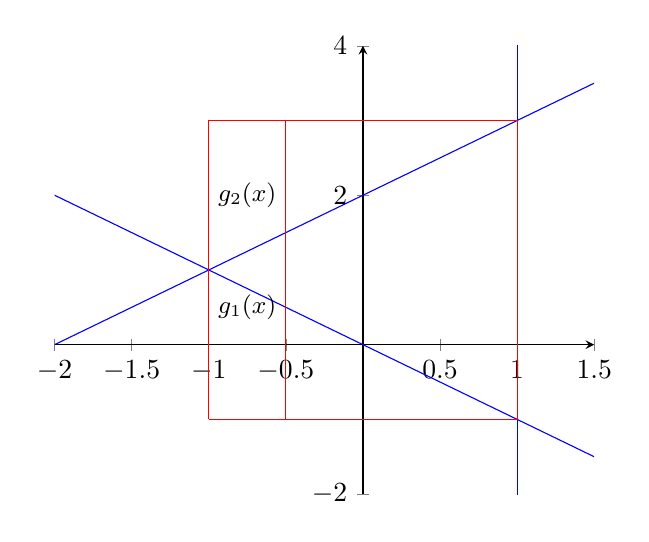
\begin{tikzpicture}
			\begin{axis}[
				xmin= -2, xmax= 1.5,
				ymin= -2, ymax = 4,
				axis lines = middle
			]
				\addplot[color=blue,domain=-10:10, samples=100]{x+2};
				\addplot[color=blue,domain=-10:10, samples=100]{-x};
				\draw[color=blue] (1,-10) -- (1,10);
				\draw[color=red] (-1,-1) -- (-1,3) -- (1,3) --(1,-1) -- (-1,-1);
				\draw[color=red] (-0.5,3) -- (-0.5,-1);
				\node at (-0.75,2) {\small$g_2(x)$};
				\node at (-0.75,0.5) {\small$g_1(x)$};

			\end{axis}
		\end{tikzpicture}
		\caption{}
	\end{figure}
	

	$f: \R^2 \longrightarrow \R$, $(x,y) \longmapsto xy$ est continue sur $\ds{\R^2}$ avec $\ds{T\subset[-1,1]\times [-1,3]}$.\\

	Ainsi : $\ds{\iint\limits_{T}^{} xy \  d x dy = \int\limits_{-1}^{1} \left( \int\limits_{g_1(x)}^{g_2(x)} xy \  d y  \right)  \  d x = \int\limits_{-1}^{1} \left( \int\limits_{G_1(y)}^{1} xy \  d x  \right)  \  d y + \int\limits_{-1}^{1} \left( \int\limits_{G_2(y)}^{1} xy \  d x  \right)  \  d y   }$

	Or $\ds{G_1(y)= -y}$ et $\ds{G_2(y)=y-2}$ donc on a : \\
	\centerline{$\ds{\int\limits_{-1}^{1} \left( \int\limits_{-x}^{x+2} xy \  d y  \right)  \  d x = \int\limits_{-1}^{1} \frac{1}{2}xy^2]\limits_{-x}^{[x+2]} \  d x  = \int\limits_{-1}^{1} \frac{1}{2}x(x+2)^2-\frac{1}{2}x^3 \  d x = \int\limits_{-1}^{1} 2x^2+2x \  d x = \frac{4}{3}}$}
		
\newpage
	\section{Exercise 58}

	\begin{figure}[ht!]
		\centering
		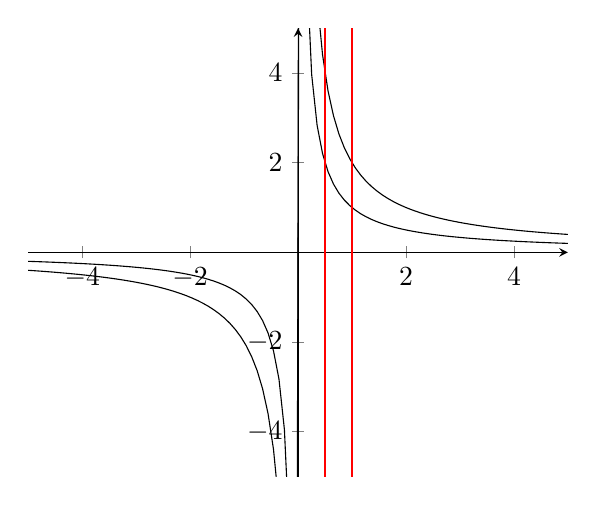
\begin{tikzpicture}
			\begin{axis}[
				xmin= -5, xmax= 5,
				ymin= -5, ymax = 5,
				axis lines = middle,
			]
				\addplot[domain=-5:5, samples=100]{1/x};
				\addplot[domain=-5:5, samples=100]{2/x};
				\draw[color=red] (0.5,-5) --(0.5,5);
				\draw[color=red] (1,-5) -- (1,5);
			\end{axis}
		\end{tikzpicture}
		\caption{}
	\end{figure}

	\begin{align*}
	\int\limits_{\frac{\pi}{6}}^{\frac{\pi}{3}} \left( \int\limits_{\frac{1}{x}}^{\frac{2}{x}} x \sin(\frac{\pi}{2}xy+x) \  d y  \right)  \  d x =& \int\limits_{\frac{\pi}{6}}^{\frac{\pi}{3}} -\frac{2}{\pi}\cos\left( \frac{\pi}{2}xy+x \right) \Bigg]\limits_{\frac{1}{x}}^{\frac{2}{x}} \  d x \\
	&= \int\limits_{\frac{\pi}{6}}^{\frac{\pi}{3}} \frac{2}{\pi}\cos(x)+\frac{2}{\pi}\sin(x) \  d x\\
	&= \frac{2}{\pi}\sin (x)-\frac{2}{\pi}\cos(x)\Big] \int\limits_{\frac{\pi}{6}}^{\frac{\pi}{3}}\\
	&= \frac{\sqrt{3} }{\pi} + \frac{1}{\pi} + \frac{1}{\pi} +\frac{\sqrt{3} }{\pi} = \frac{2\sqrt{3} -2}{\pi}
	\end{align*}

	$f: \R^2 \longrightarrow \R$, $ (x,y) \longmapsto x \sin\left( \frac{\pi}{2}xy+x \right) $ est continue sur $\ds{\R}$ donc ses intégrales éxistent 

	\section{Calcul asymptotique et développement limités}

	\subsection{Exercise 60}

	

	\subsection{Exercise 61}

	On pose $\ds{X=\ln x}$ alors on transforme les quantités : \\
	\centerline{$\ds{x=e^u, \quad \exp(\sqrt{u} ), \quad \exp\left( u^2 \right), \quad \exp(\exp(u)) }$}

	\subsection{Exercise 62}

	On cherche le développement limité de $f: \R \longrightarrow \R$, $x \longmapsto (\sin x)\ln(1+x)$ en 0 d'ordre $\ds{4}$

	$\ds{\sin x = x - \frac{1}{6}x^3 +o(x^4)}$\\
	$\ds{\ln(1+x)= x -\frac{1}{2}x^2+ \frac{1}{3}x^3 - \frac{1}{4}x^4 + o(x^4)}$\\
	Donc par produit de développement limités :\\
	$\ds{(\sin x)\ln(x+1)= \left( x -\frac{1}{2}x^2+ \frac{1}{3}x^3 - \frac{1}{4}x^4  \right) x -\frac{1}{6}\left( x -\frac{1}{2}x^2+ \frac{1}{3}x^3 - \frac{1}{4}x^4  \right)x^3+o(x^4) }$

	On cherche le développement limité de $f: \R \longrightarrow \R$, $x \longmapsto \frac{1}{1+x+x^2}$ en 0 d'ordre $\ds{4}$

	$\ds{\frac{1}{1+x+x^2}= 1 - x +x^3 -x^4 + o(x^4) }$

	\begin{dent}{Note:} on peut effectuer par substitution $\ds{u=x+x^2}$ pour calculer le développement limité de $\ds{\frac{1}{1+u}}$

		On s'assure que pour $\ds{x\to 0}$, on a $\ds{u\to 0}$. Ainsi par composition:

		$\ds{\frac{1}{1+x}= 1-x+x^2-x^3 + x^4+ o(x^4)}$ et $\ds{x+x^2}= x+x^2 +o(x^4)$ \\
		On a  alors $\ds{\frac{1}{1+x+x^2}= 1+ \left( x+x^2 \right) + \left( x+x^2 \right)^2 + \left( x+x^2 \right) ^3 +\left( x+x^2 \right) ^4 + o(x^4) }$

		Ainsi en développant : $\ds{\frac{1}{1+x+x^2}= 1-x+x^3-x^4 +o(x^4)}$
		
	\end{dent}

	On cherche le développement limité de $f: \R \longrightarrow \R$, $x \longmapsto \exp(\sin x)$ en 0 d'ordre $\ds{3}$\\
	En prenant $\ds{u=\sin x}$, on s'assure que quand $\ds{x\to 0}$, $\ds{u\to 0}$ on applique la composition :\\
	$\ds{\sin x = x -\frac{1}{6}x^3 +o (x^3)}$ et $\ds{e^x}=1 +x+x^2+x^3+o(x^3))$

	On retrouve : $\ds{\exp(\sin x)= 1+ \left( x-\frac{1}{6}x^3 \right) +\left( x-\frac{1}{6}x^3 \right) ^2 + \left( x-\frac{1}{6}x^3 \right) ^3}$\\

	Ainsi $\ds{\exp(\sin x)= 1+x+x^2+\frac{5}{6}x^3 +o(x^3)}$

\end{document}
